\documentclass[aspectratio=169,11pt]{beamer}

\usetheme{Madrid}
\setbeamertemplate{navigation symbols}{}

\usepackage[utf8]{inputenc}
\usepackage[T1]{fontenc}
\usepackage{lmodern}
\usepackage{graphicx}
\usepackage{booktabs}
\usepackage{amsmath}
\usepackage{array}
\usepackage{xcolor}
\usecolortheme{default}
\newcommand{\titlecite}[2]{\texorpdfstring{\href{#1}{[#2]}}{[#2]}}

\title[DHVT vs CNN]{AlexNet et DHVT pour la classification d'images}
\author[Haobo \& Zhenyu]{Haobo YANG 22513870 \\ Zhenyu XU 22508276}
\institute{Universit\'e Paris Cit\'e}
\date{Ann\'ee universitaire 2025--2026}

\begin{document}

\begin{frame}
    \titlepage
\end{frame}

\begin{frame}{Plan}
    \tableofcontents
\end{frame}

\section{Objectif}

\begin{frame}{Question du projet}
    \begin{itemize}
        \item On compare un \textbf{CNN classique} et une architecture \textbf{de type transformer} sur des petits jeux de donn\'ees d'images.
        \item Le baseline est \textbf{AlexNet} ; le mod\`ele principal est \textbf{DHVT}.
        \item La question centrale est simple : \textbf{comment rendre un ViT plus efficace sur un petit dataset ?}
    \end{itemize}
\end{frame}

\section{Architecture}

\begin{frame}{Point de d\'epart : le CNN \titlecite{https://papers.nips.cc/paper_files/paper/2012/hash/c399862d3b9d6b76c8436e924a68c45b-Abstract.html}{1}}
    \centering
    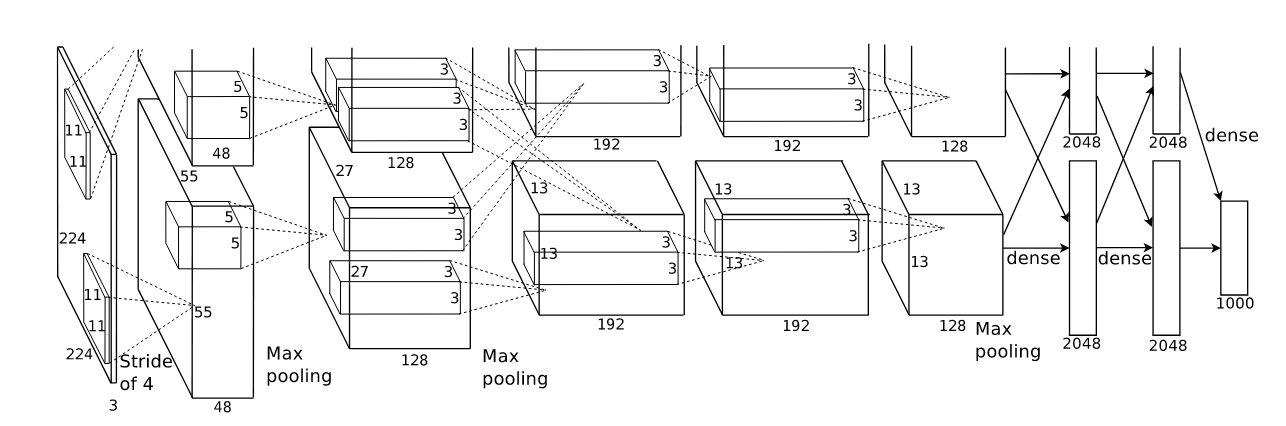
\includegraphics[height=0.4\textheight,keepaspectratio]{architecture/cnn.png}

    \vspace{0.25cm}
    \textbf{AlexNet}
    \begin{itemize}
        \item Il utilise des \textbf{convolutions}.
        \item Il apprend d'abord des \textbf{motifs locaux}.
        \item Limite : il capture moins bien les relations \textbf{globales}.
    \end{itemize}

    \vspace{0.1cm}
    \scriptsize 

    \[
    Y_{i,j}=\sum_u\sum_v K_{u,v}X_{i+u,j+v}
    \]
\end{frame}


\begin{frame}{Vue d'ensemble de DHVT \titlecite{https://arxiv.org/abs/2010.11929}{2} \titlecite{https://arxiv.org/abs/2203.16353}{3}}
    \centering
    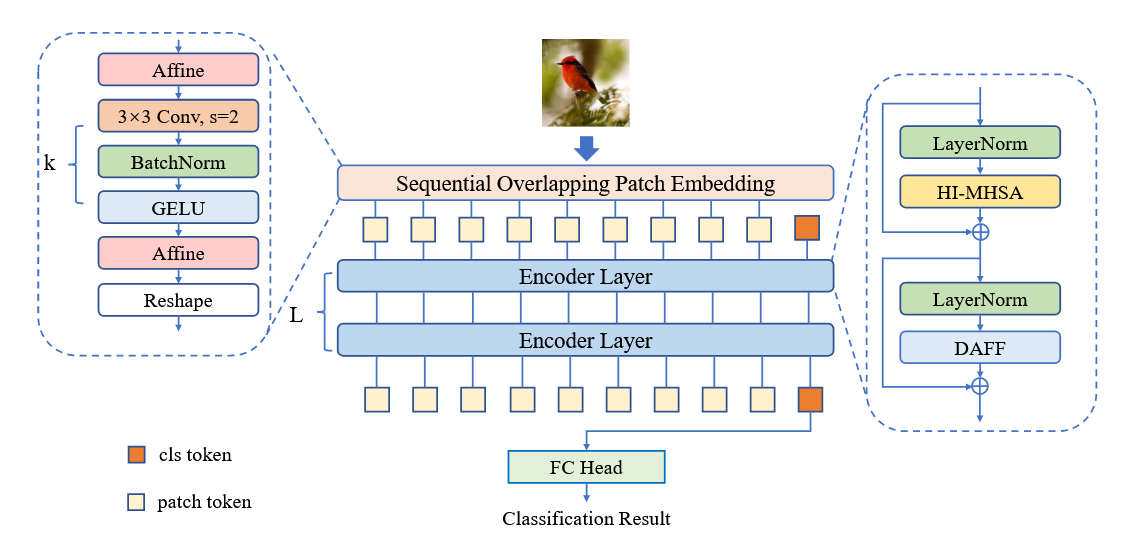
\includegraphics[width=0.82\linewidth,height=0.34\textheight,keepaspectratio]{architecture/DHVT.png}

    \vspace{0.15cm}
    \begin{itemize}
        \item \hyperlink{app:sope}{\textbf{SOPE}} $\rightarrow$ ajoute une entr\'ee de type plus \textbf{convolutionnelle}, donc plus locale.
        \item \hyperlink{app:himhsa}{\textbf{HI-MHSA}} $\rightarrow$ garde la partie \textbf{globale} du transformer.
        \item \hyperlink{app:daff}{\textbf{DAFF}} $\rightarrow$ remet de la \textbf{convolution} dans le bloc interne, donc une logique plus proche du CNN.
    \end{itemize}
\end{frame}

\begin{frame}{R\'esum\'e de la structure}
    \begin{table}
        \centering
        \begin{tabular}{p{2.2cm}p{3.4cm}p{6.5cm}}
            \toprule
            Module & Ce qui change & Pourquoi c'est utile \\
            \midrule
            \textcolor{blue!70!black}{\hyperlink{app:sope}{SOPE}} & Nouvelle entr\'ee & Garde mieux l'information locale \\
            \textcolor{blue!70!black}{\hyperlink{app:himhsa}{HI-MHSA}} & Nouvelle attention & Organise mieux l'information globale \\
            \textcolor{blue!70!black}{\hyperlink{app:daff}{DAFF}} & Nouveau bloc interne & Rajoute du local dans le transformer \\
            \bottomrule
        \end{tabular}
    \end{table}

    \vspace{0.25cm}
    \begin{itemize}
        \item En r\'esum\'e, \textbf{DHVT garde le global du transformer}.
        \item Mais il \textbf{r\'ecup\`ere aussi le local}, ce qui est utile sur les petites images.
    \end{itemize}
\end{frame}

\section{R\'esultats}

\begin{frame}{R\'esultat principal}
    \begin{table}
        \centering
        \begin{tabular}{>{\raggedright\arraybackslash}p{4.7cm}cc}
            \toprule
            Mesure & CIFAR-10 & CIFAR-100 \\
            \midrule
            Accuracy AlexNet / DHVT & 0.6848 / 0.7762 & 0.2856 / 0.5012 \\
            \'Ecart d'accuracy & +0.0914 & +0.2156 \\
            F1 macro AlexNet / DHVT & 0.6814 / 0.7759 & 0.2713 / 0.4958 \\
            Param\`etres AlexNet / DHVT & 58.32M / 6.80M & 58.69M / 6.81M \\
            \bottomrule
        \end{tabular}
    \end{table}

    \vspace{0.25cm}
    \begin{itemize}
        \item DHVT est \textbf{meilleur sur les deux jeux de donn\'ees}.
        \item L'\'ecart devient \textbf{beaucoup plus grand sur CIFAR-100}.
        \item Le mod\`ele est aussi \textbf{bien plus compact} qu'AlexNet.
    \end{itemize}
\end{frame}

\begin{frame}{Les figures confirment la conclusion}
    \centering
    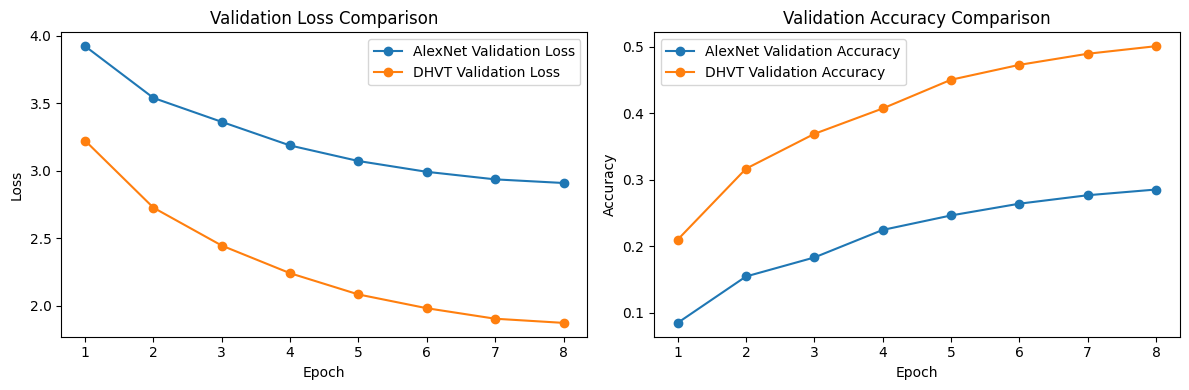
\includegraphics[width=0.88\linewidth,height=0.42\textheight,keepaspectratio]{figures/validation_curves_cifar100.png}

    \vspace{0.25cm}
    \begin{itemize}
        \item C'est la figure la plus importante car \textbf{CIFAR-100} est le cas le plus difficile.
        \item DHVT apprend \textbf{plus vite}.
        \item Il reste \textbf{au-dessus d'AlexNet} pendant tout l'entra\^\i nement.
        \item Donc son avantage n'appara\^\i t pas seulement \`a la fin.
    \end{itemize}
\end{frame}

\begin{frame}{La confiance des pr\'edictions est plus coh\'erente}
    \centering
    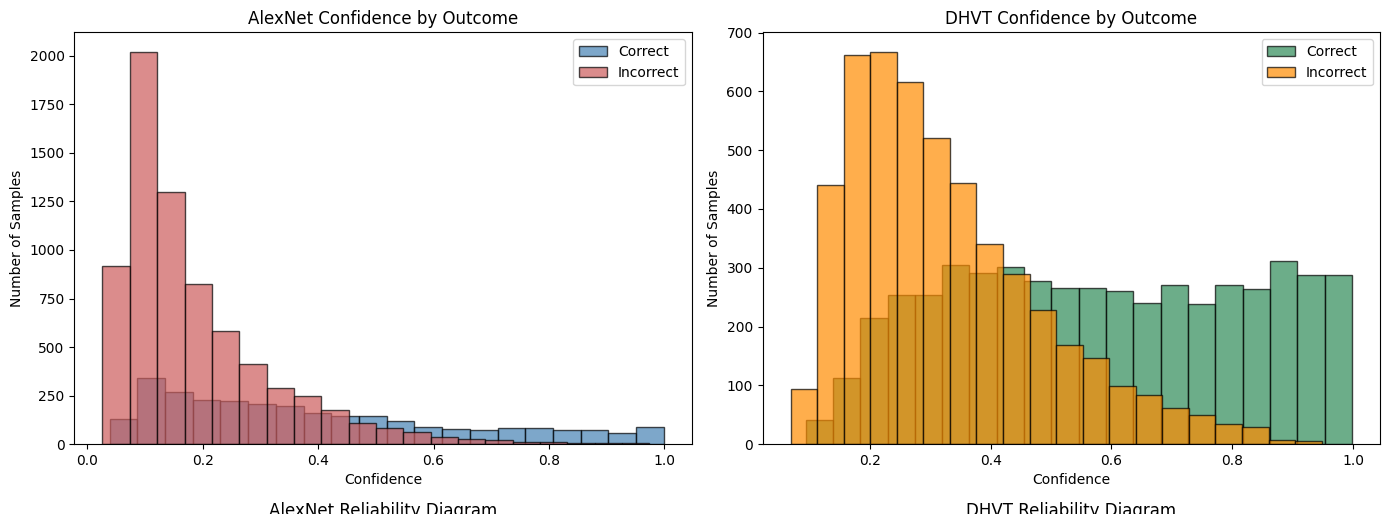
\includegraphics[width=0.88\linewidth,height=0.42\textheight,keepaspectratio]{figures/confidence_distribution_cifar100_top.png}

    \vspace{0.25cm}
    \begin{itemize}
        \item DHVT s\'epare mieux les \textbf{bonnes} et les \textbf{mauvaises} pr\'edictions.
        \item Donc ses scores de confiance sont plus \textbf{coh\'erents}.
        \item Ce n'est pas seulement un meilleur score final.
    \end{itemize}
\end{frame}

\begin{frame}{Le gain n'est pas limit\'e \`a quelques classes}
    \centering
    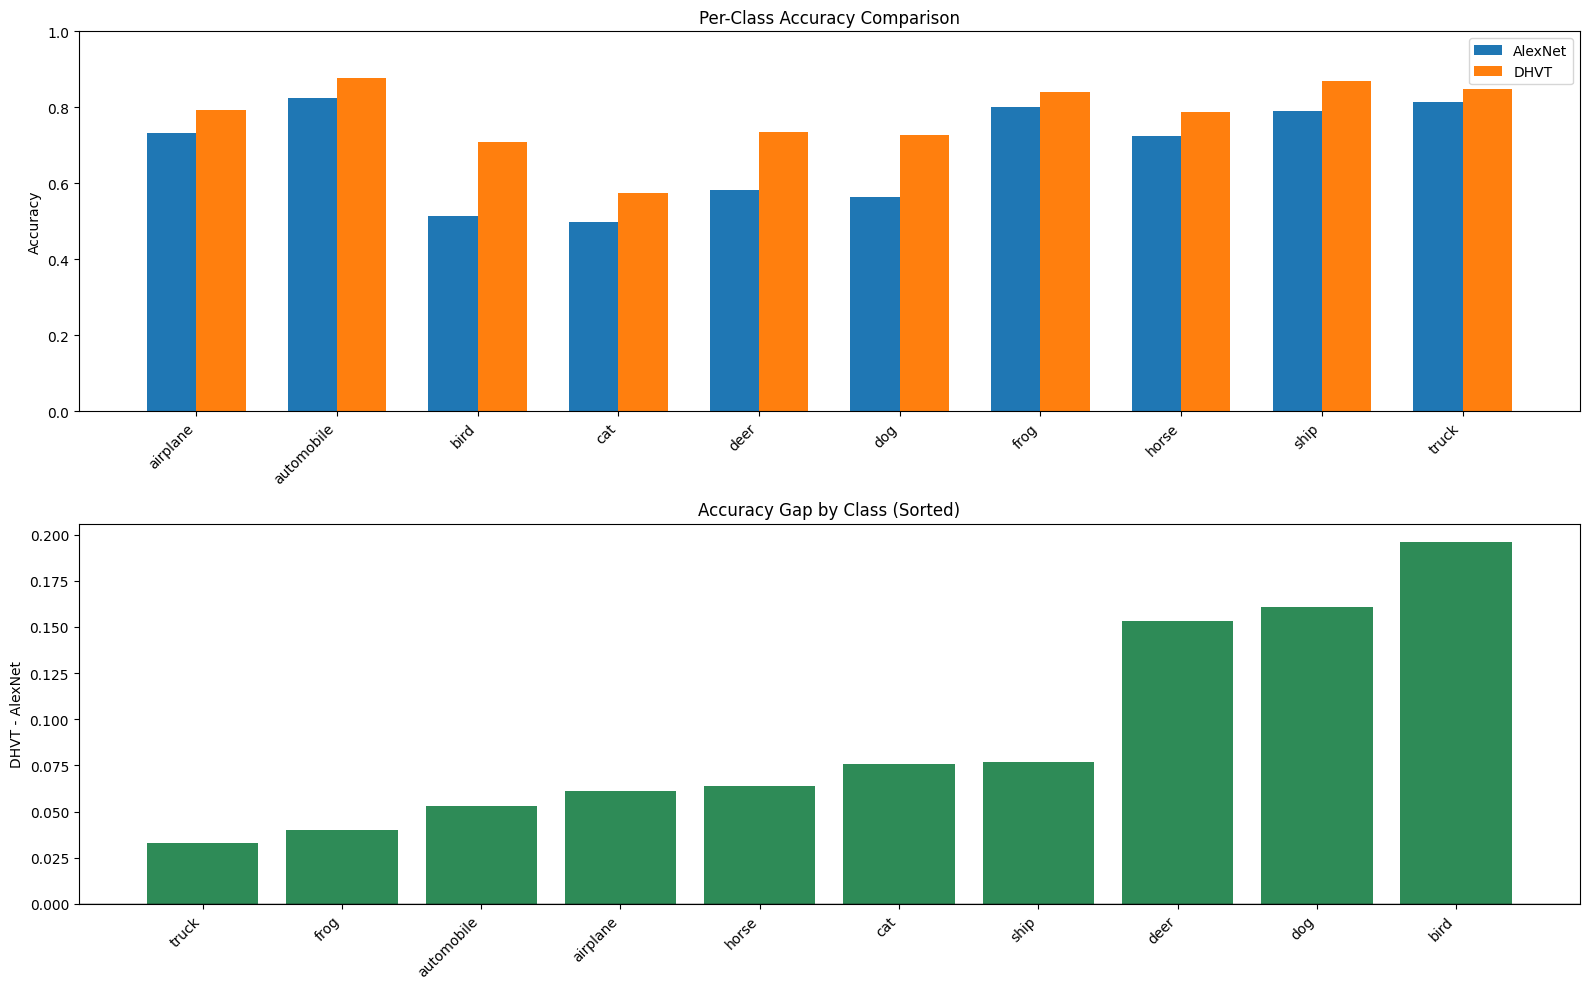
\includegraphics[width=0.88\linewidth,height=0.42\textheight,keepaspectratio]{figures/per_class_accuracy_gap.png}

    \vspace{0.25cm}
    \begin{itemize}
        \item L'\'ecart entre DHVT et AlexNet est \textbf{positif pour toutes les classes}.
        \item Le gain n'est donc pas limit\'e \`a quelques classes faciles.
        \item L'avantage de DHVT est \textbf{global}.
    \end{itemize}
\end{frame}

\begin{frame}{Exemples d'erreurs de classification}
    \begin{columns}[c, onlytextwidth]
        \begin{column}{0.60\linewidth}
            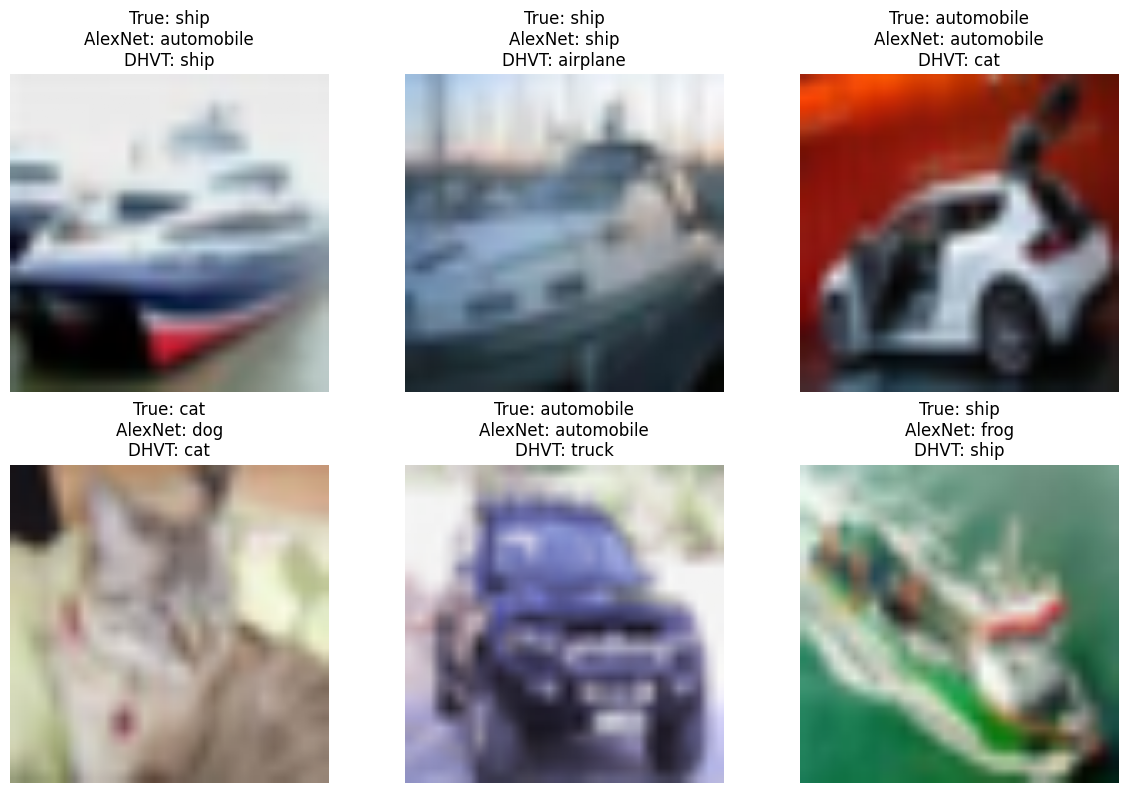
\includegraphics[width=\linewidth]{figures/misclassified_examples.png}
        \end{column}
        \begin{column}{0.4\linewidth}
        	\vfill
            \begin{itemize}
                \item On voit ici des \textbf{cas difficiles}.
                \item Dans plusieurs exemples, \textbf{DHVT corrige} une erreur d'AlexNet.
                \item Les erreurs restantes viennent souvent d'images \textbf{petites} ou \textbf{ambigu\"es}.
            \end{itemize}
            \vfill
        \end{column}
    \end{columns}
\end{frame}

\begin{frame}{Cartes d'attention de DHVT}
    \begin{columns}[c,onlytextwidth]
        \begin{column}{0.5\textwidth}
            \centering
            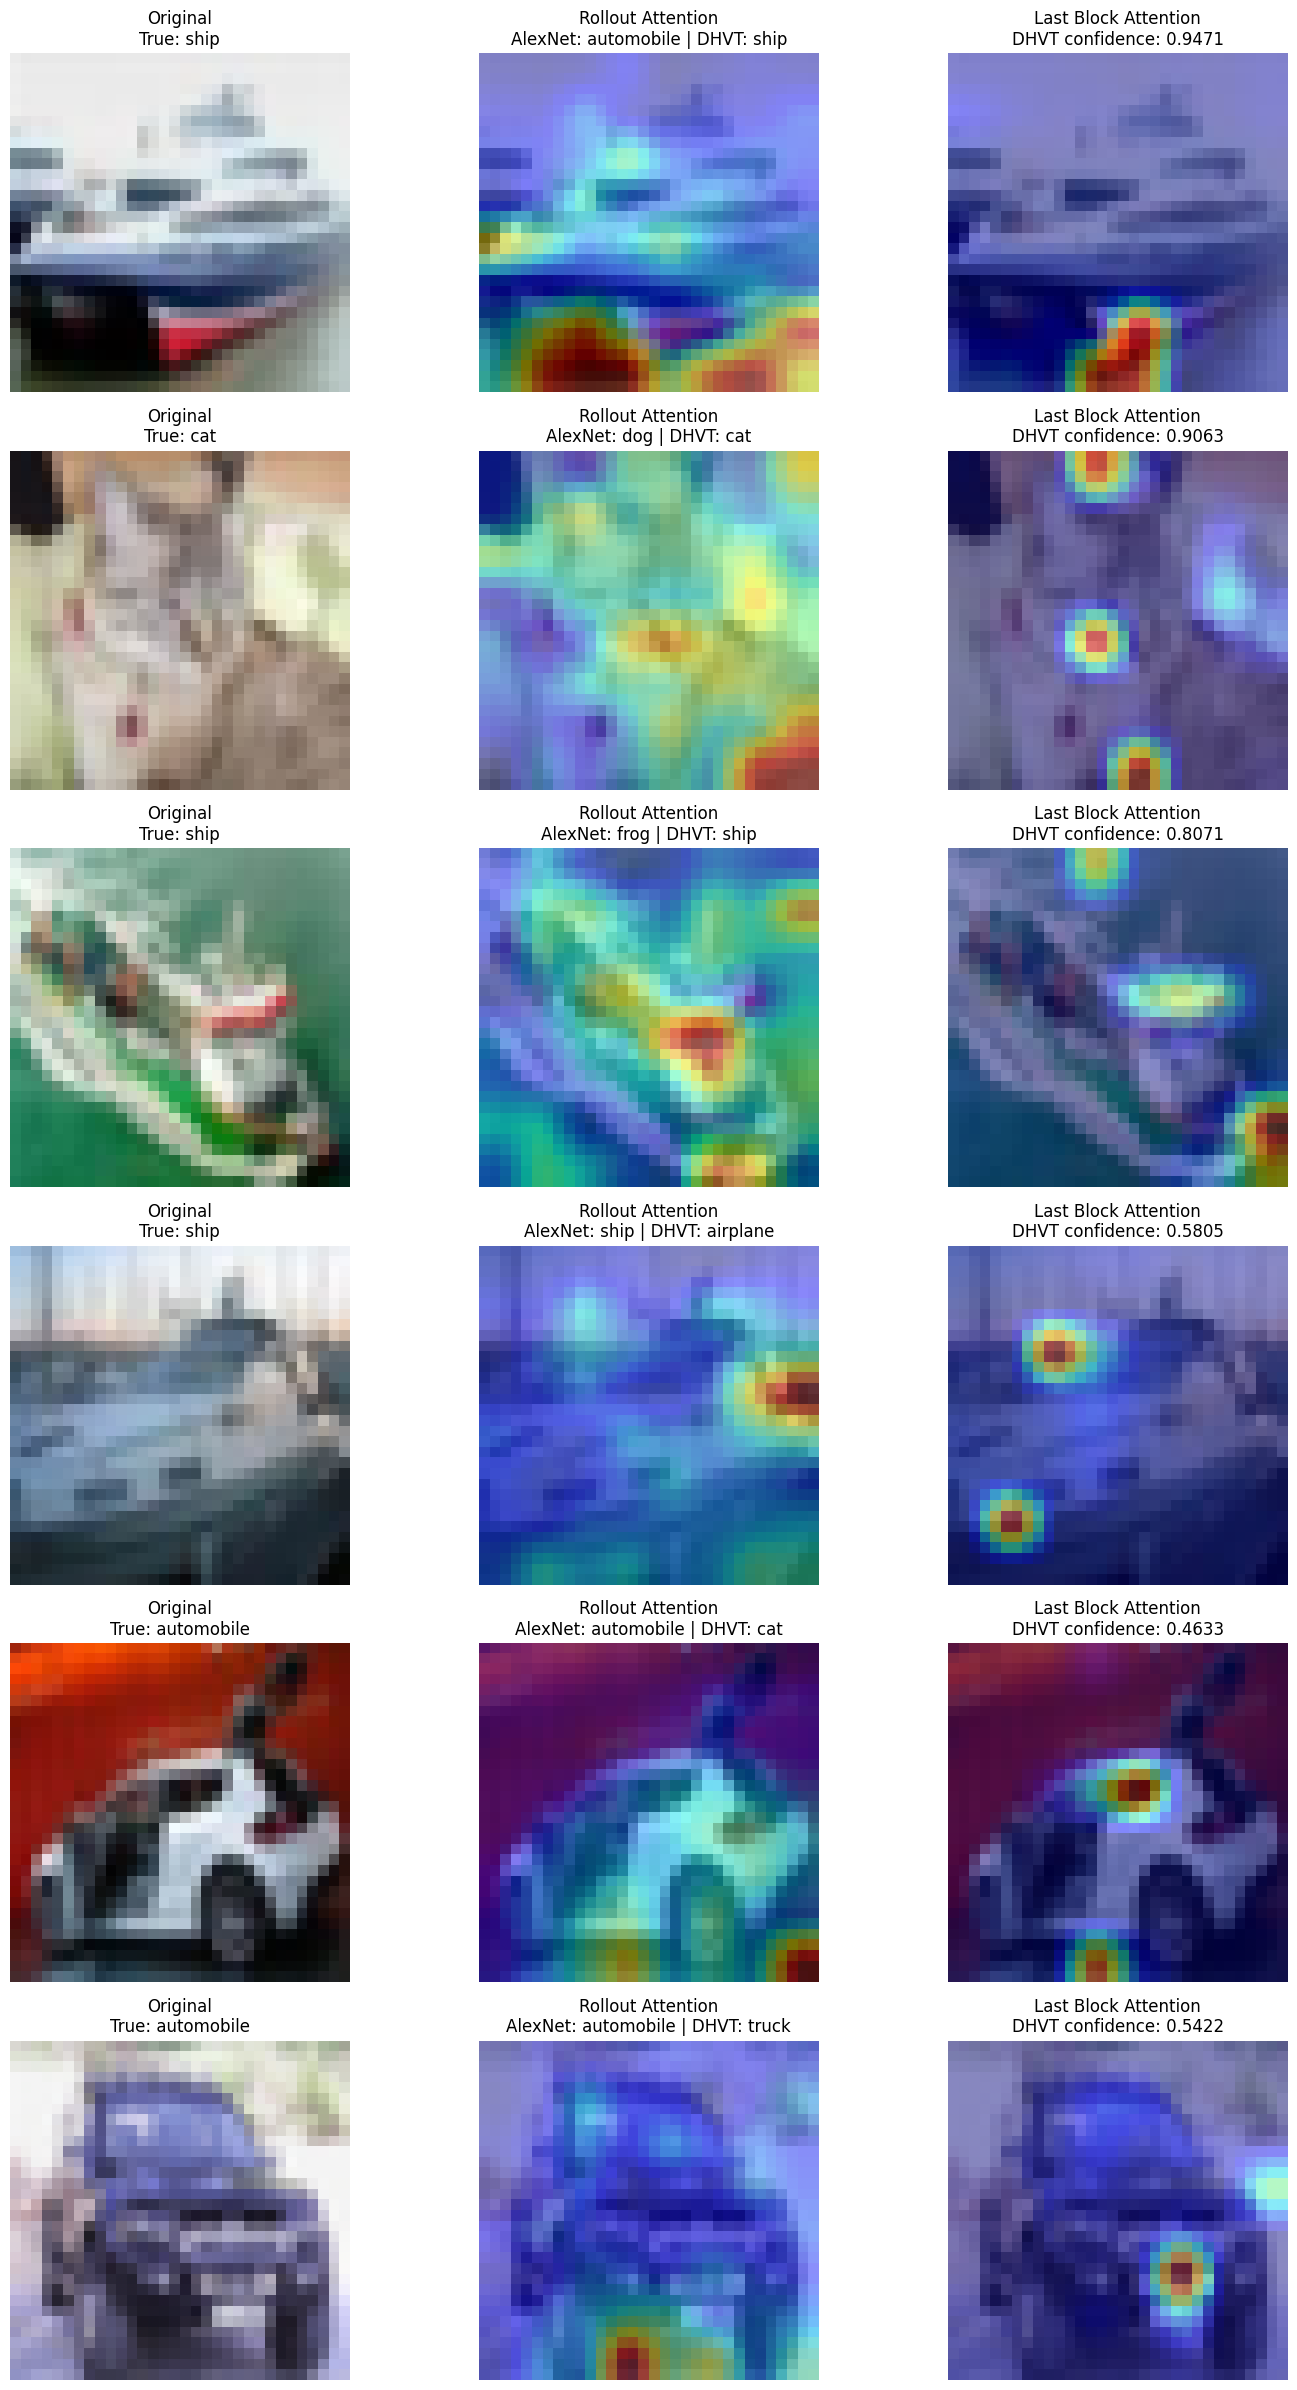
\includegraphics[width=\linewidth,height=0.8\textheight,keepaspectratio]{figures/dhvt_attention_visualization.png}
        \end{column}
        \begin{column}{0.5\textwidth}
            \begin{itemize}
                \item Les cartes montrent \textbf{o\`u DHVT regarde}.
                \item Sur les bons exemples, l'attention vise souvent l'\textbf{objet principal}.
                \item Sur les erreurs, elle est plus \textbf{diffuse}.
            \end{itemize}
        \end{column}
    \end{columns}
\end{frame}

\begin{frame}{R\'esultats sur les variantes de CIFAR-100}
    \begin{table}
        \centering
        \begin{tabular}{p{3.2cm}ccc}
            \toprule
            Variante & AlexNet acc. & DHVT acc. & \'Ecart \\
            \midrule
            clean & 0.2694 & 0.5167 & +0.2472 \\
            texture & 0.2583 & 0.4278 & +0.1694 \\
            damaged\_occluded & 0.2944 & 0.4222 & +0.1278 \\
            long\_range & 0.3333 & 0.4472 & +0.1139 \\
            \bottomrule
        \end{tabular}
    \end{table}

    \vspace{0.25cm}
    \begin{itemize}
        \item DHVT reste \textbf{meilleur sur toutes les variantes}.
        \item L'avantage est maximal sur \texttt{clean}.
        \item Mais il reste pr\'esent sur toutes les autres variantes.
        \item Donc le gain n'est pas limit\'e \`a un seul type de difficult\'e.
    \end{itemize}
\end{frame}

\section{Conclusion}

\begin{frame}{Conclusion}
    \begin{itemize}
        \item Le \textbf{CNN} est fort pour le \textbf{local}.
        \item Le \textbf{ViT} est fort pour le \textbf{global}.
        \item \textbf{DHVT} essaie de combiner les deux.
        \item Dans nos exp\'eriences, cela donne \textbf{de meilleurs r\'esultats qu'AlexNet}, surtout sur les cas difficiles.
    \end{itemize}
\end{frame}

\begin{frame}{R\'ef\'erences}
    \small
    \begin{itemize}
        \item [1] Krizhevsky, A., Sutskever, I., and Hinton, G. E. \textit{ImageNet Classification with Deep Convolutional Neural Networks}. Advances in Neural Information Processing Systems (NeurIPS), 2012.
        \item [2] Dosovitskiy, A. et al. \textit{An Image is Worth 16x16 Words: Transformers for Image Recognition at Scale}. International Conference on Learning Representations (ICLR), 2021.
        \item [3] Lu, Y. et al. \textit{Bridging the Gap Between Vision Transformers and Convolutional Neural Networks on Small Datasets}. arXiv preprint arXiv:2203.16353, 2022.
    \end{itemize}
\end{frame}

\begin{frame}{Merci}
    \centering
    \Large Merci pour votre attention

    \vspace{0.4cm}
    \normalsize Questions ?
\end{frame}

\appendix
\section{Annexe}

\begin{frame}{Annexe : SOPE}
    \hypertarget{app:sope}{}
    \centering
    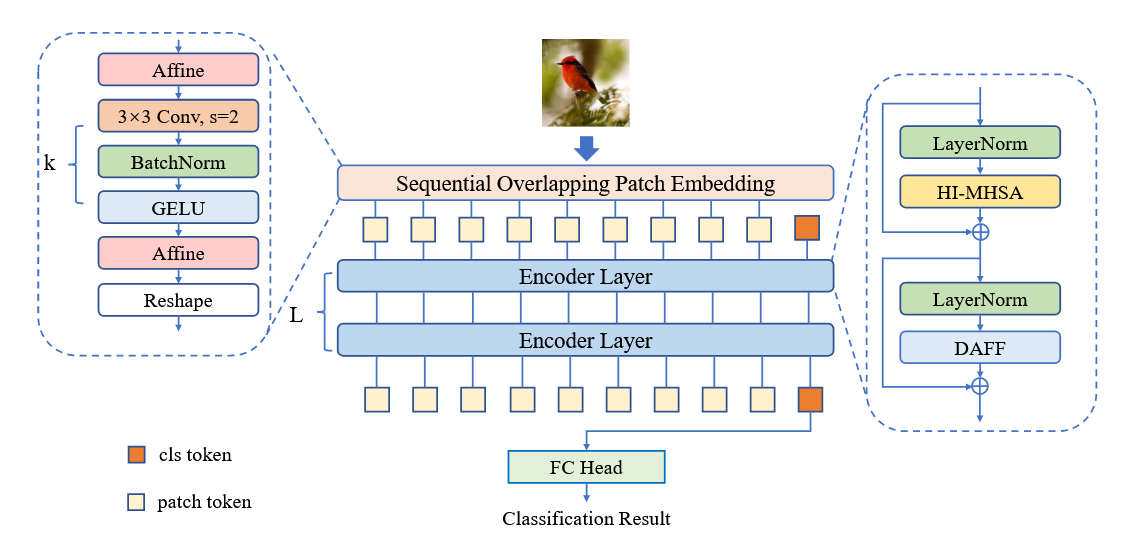
\includegraphics[width=0.88\linewidth,height=0.56\textheight,keepaspectratio]{architecture/DHVT.png}

    \vspace{0.2cm}
    \begin{itemize}
        \item SOPE remplace l'entr\'ee par patches trop directe.
        \item L'id\'ee est de garder plus d'information locale d\`es le d\'ebut.
        \item Donc les tokens d'entr\'ee sont plus adapt\'es aux petites images.
    \end{itemize}
\end{frame}

\begin{frame}{Annexe : HI-MHSA}
    \hypertarget{app:himhsa}{}
    \centering
    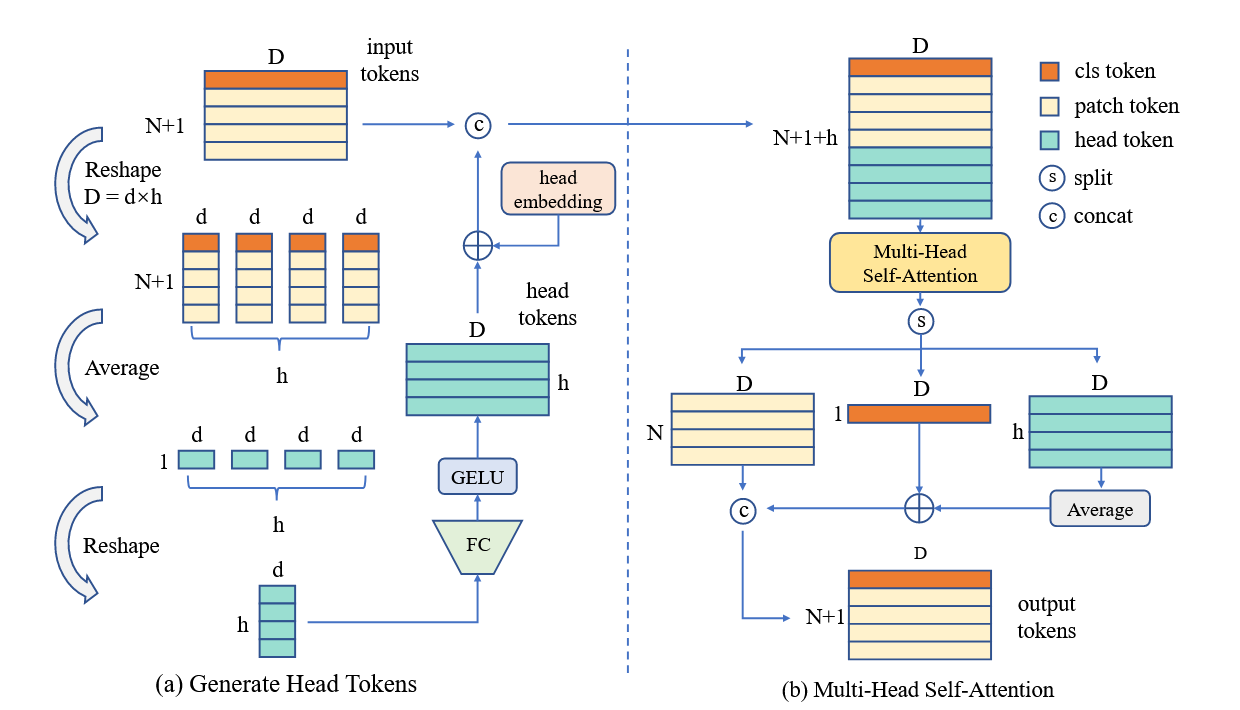
\includegraphics[width=0.88\linewidth,height=0.56\textheight,keepaspectratio]{architecture/HI-MHSA.png}

    \vspace{0.2cm}
    \begin{itemize}
        \item HI-MHSA modifie le bloc d'attention.
        \item Les \textit{head tokens} aident \`a mieux organiser l'information globale.
        \item Le but est d'obtenir une meilleure repr\'esentation finale pour la classification.
    \end{itemize}
\end{frame}

\begin{frame}{Annexe : DAFF}
    \hypertarget{app:daff}{}
    \centering
    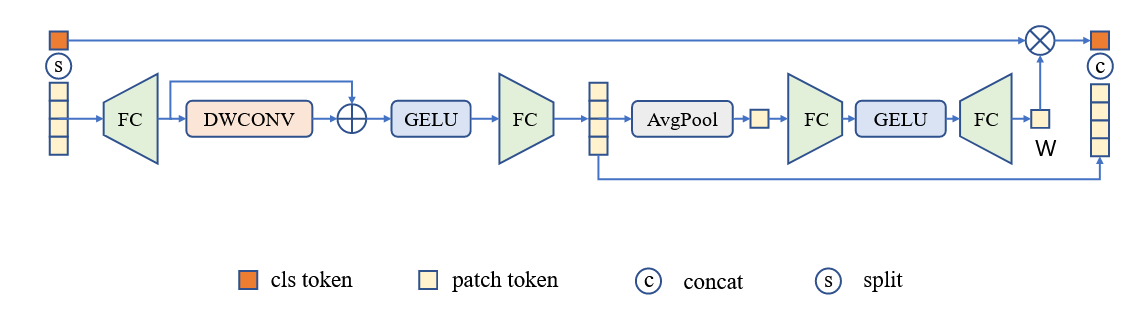
\includegraphics[width=0.88\linewidth,height=0.56\textheight,keepaspectratio]{architecture/DAFF.png}

    \vspace{0.2cm}
    \begin{itemize}
        \item DAFF remplace le FFN standard.
        \item Il ajoute une partie locale dans le bloc transformer.
        \item Cela aide DHVT \`a combiner information locale et information globale.
    \end{itemize}
\end{frame}

\end{document}
